% ============================================================
%  Numerical Processing of Financial Data — Project Report
%  Romain ETIENNE & Anirudh SUDHIR — Polytechnique/HEC Data & Finance
%
%  Compile with:  pdflatex main.tex  (run twice for correct refs)
% ============================================================

\documentclass[10pt, a4paper]{article}

% ---------- Encoding & fonts ----------
\usepackage[T1]{fontenc}
\usepackage[utf8]{inputenc}
\usepackage{lmodern}
\usepackage{microtype}

% ---------- Layout ----------
\usepackage[top=2.2cm, bottom=2.2cm, left=2.2cm, right=2.2cm]{geometry}
\usepackage{parskip}
\setlength{\parskip}{4pt}
\usepackage{fancyhdr}
\usepackage{titlesec}
\usepackage{enumitem}

% ---------- Math ----------
\usepackage{amsmath, amssymb}

% ---------- Graphics & tables ----------
\usepackage{graphicx}
\usepackage{booktabs}
\usepackage{array}
\usepackage{float}
\usepackage{caption}
\captionsetup{font=small, skip=4pt}
\usepackage{subcaption}
\usepackage{xcolor}

% ---------- Links ----------
\usepackage[hidelinks]{hyperref}

% ---------- Figures path ----------
\graphicspath{{figures/}}

% ---------- Section spacing ----------
\titlespacing*{\section}{0pt}{1.0em}{0.3em}
\titlespacing*{\subsection}{0pt}{0.7em}{0.2em}

% ============================================================
\begin{document}

% ======================== TITLE ========================
\begin{center}
  {\small \scshape \'Ecole Polytechnique -- HEC Paris \quad|\quad Master Data \& Finance}\\[0.4em]
  {\LARGE\bfseries Risk and Performance of a Dynamic Markowitz Portfolio\\[0.2em]
   on CAC~40 Constituents}\\[0.6em]
  {\normalsize
    Romain \textsc{Etienne} \quad\textbullet\quad Anirudh \textsc{Sudhir}\\[0.2em]
    Supervisor: M.~Garcin \quad|\quad March 2025}
\end{center}
\rule{\linewidth}{0.5pt}

\pagestyle{fancy}
\fancyhf{}
\fancyhead[L]{\small Numerical Processing of Financial Data}
\fancyhead[R]{\small Etienne \& Sudhir}
\fancyfoot[C]{\thepage}
\renewcommand{\headrulewidth}{0.4pt}

% ======================== ABSTRACT ========================
\begin{abstract}
\noindent
We construct and evaluate a daily-rebalanced Markowitz portfolio on ten diversified
CAC~40 constituents using one-minute OHLC data (September~2022 -- February~2023,
$n=120$ trading days). Expected returns are proxied by AR(1) forecasts built from
lag-1 autocorrelations $\hat\rho_j \in [-0.168, 0.123]$. The unconstrained optimisation
produces extreme leverage ($\sum|\Omega_j| \approx 22$) that destroys capital: the
portfolio ends at $-1271.82$ (base~100) versus $+122.89$ for the equal-weight benchmark.
Ex-ante Sharpe is $0.96$ (annualised) vs.\ ex-post $0.44$; UPR~$= 0.32$; maximum
drawdown~$= -467\%$. The exercise illustrates the dangers of combining unconstrained
Markowitz with weak forecasts and full-sample covariance estimation.
\end{abstract}

% ======================== 1. DATASET ========================
\section{Dataset and Investment Universe}

The raw data consist of minute-frequency OHLC prices for all 40 CAC~40 constituents
stored as \texttt{.xlsx} files. The analysis window 13~September~2022 -- 28~February~2023
yields $n = 120$ trading days and $n-1 = 119$ daily returns per stock.
Daily closing prices are obtained by retaining the last intraday quote of each session.

We select ten liquid, sector-diversified stocks (Table~\ref{tab:tickers}).
Liquidity is confirmed by row counts $\ge 58\,000$ minute-bars (the bottom quartile
of the full CAC~40 falls below $\sim 40\,000$). At most one stock is taken per sector
to avoid systematic factor concentration.

\begin{table}[H]
\centering
\caption{Investment universe: ten CAC~40 constituents.}
\label{tab:tickers}
\small\setlength{\tabcolsep}{5pt}
\begin{tabular}{llll}
\toprule
\textbf{Ticker} & \textbf{Company} & \textbf{Sector} & \textbf{Rows} \\
\midrule
MC  & LVMH                    & Luxury Goods            & 61\,371 \\
BNP & BNP Paribas              & Banking                 & 60\,911 \\
AIR & Airbus                   & Aerospace \& Defence    & 60\,769 \\
CS  & AXA                      & Insurance               & 60\,150 \\
ORA & Orange                   & Telecoms                & 59\,821 \\
TTE & TotalEnergies            & Energy                  & 59\,410 \\
SU  & Schneider Electric       & Industrials             & 59\,394 \\
DSY & Dassault Syst\`emes      & Enterprise Software     & 59\,276 \\
SAN & Sanofi                   & Healthcare              & 58\,861 \\
MT  & ArcelorMittal            & Materials               & 58\,454 \\
\bottomrule
\end{tabular}
\end{table}

% ======================== 2. PORTFOLIO CONSTRUCTION ========================
\section{Portfolio Construction}

\subsection{Daily Returns}

Arithmetic daily returns $R_{i,j} = (P_{i,j} - P_{i-1,j})/P_{i-1,j}$ form a
$119\times10$ matrix. Returns are approximately centred at zero with occasional large
outliers (Figure~\ref{fig:returns}); concurrent spikes reflect systematic market events.

\begin{figure}[H]
  \centering
  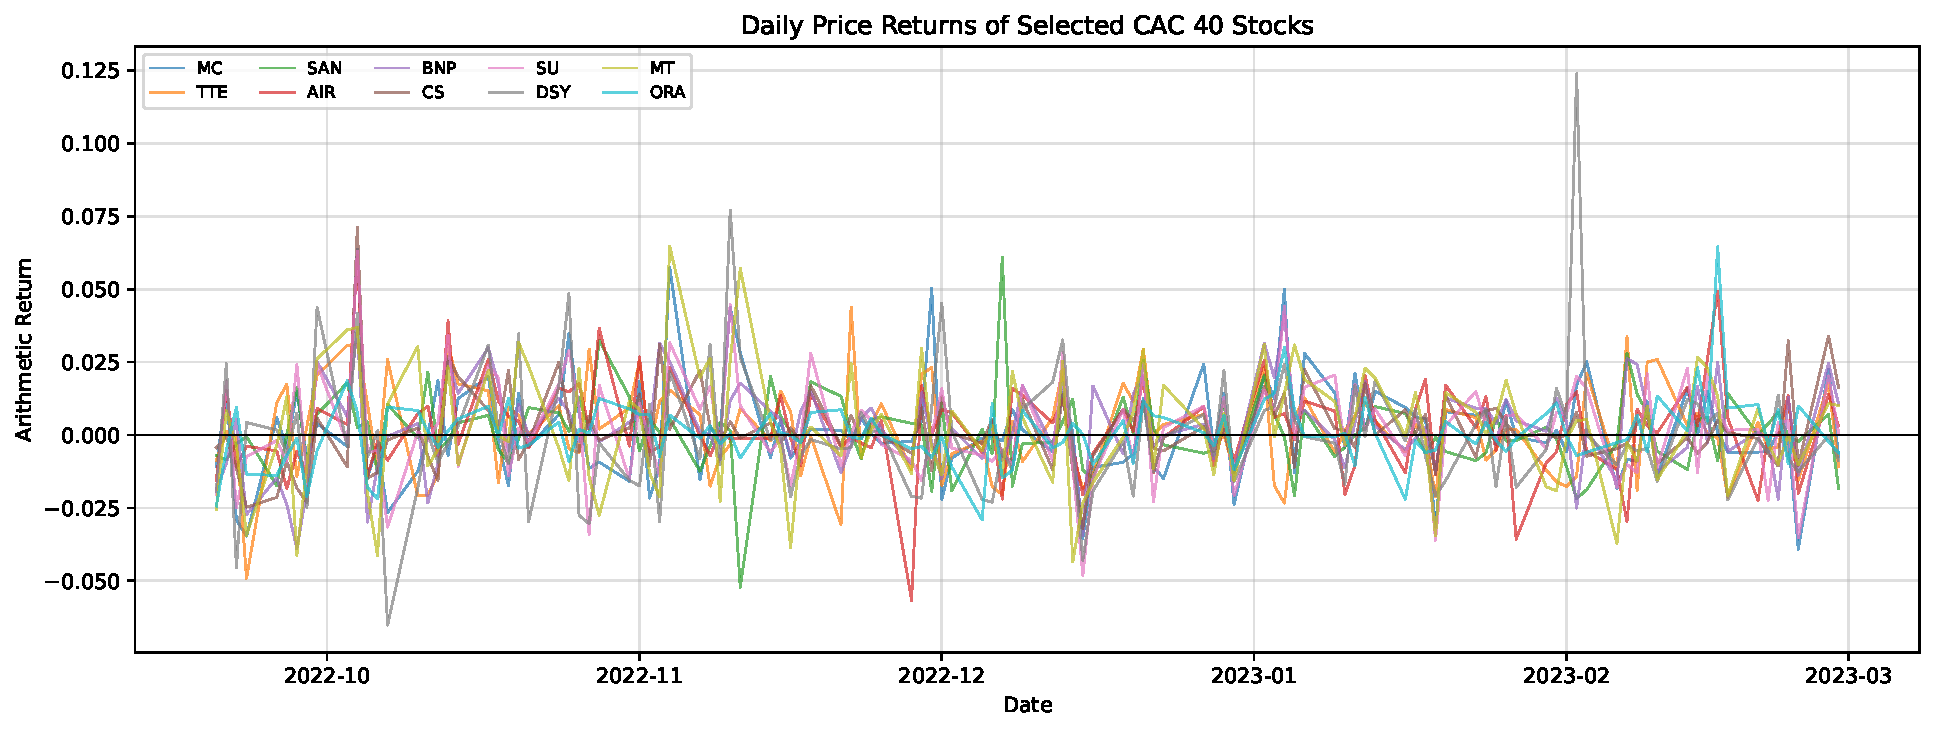
\includegraphics[width=0.92\textwidth]{fig_01_daily_returns}
  \caption{Daily arithmetic price returns for the ten selected stocks.}
  \label{fig:returns}
\end{figure}

\subsection{Correlation and Covariance}

Figure~\ref{fig:corr_cov} displays the sample correlation and covariance matrices.
All 45 pairwise correlations are positive (average~$0.29$), reflecting a shared
European equity systematic factor. The strongest links are MC--SU~(0.74) and
BNP--CS~(0.64); Sanofi and Orange show the weakest co-movements, confirming their
role as defensive diversifiers.

\begin{figure}[H]
  \centering
  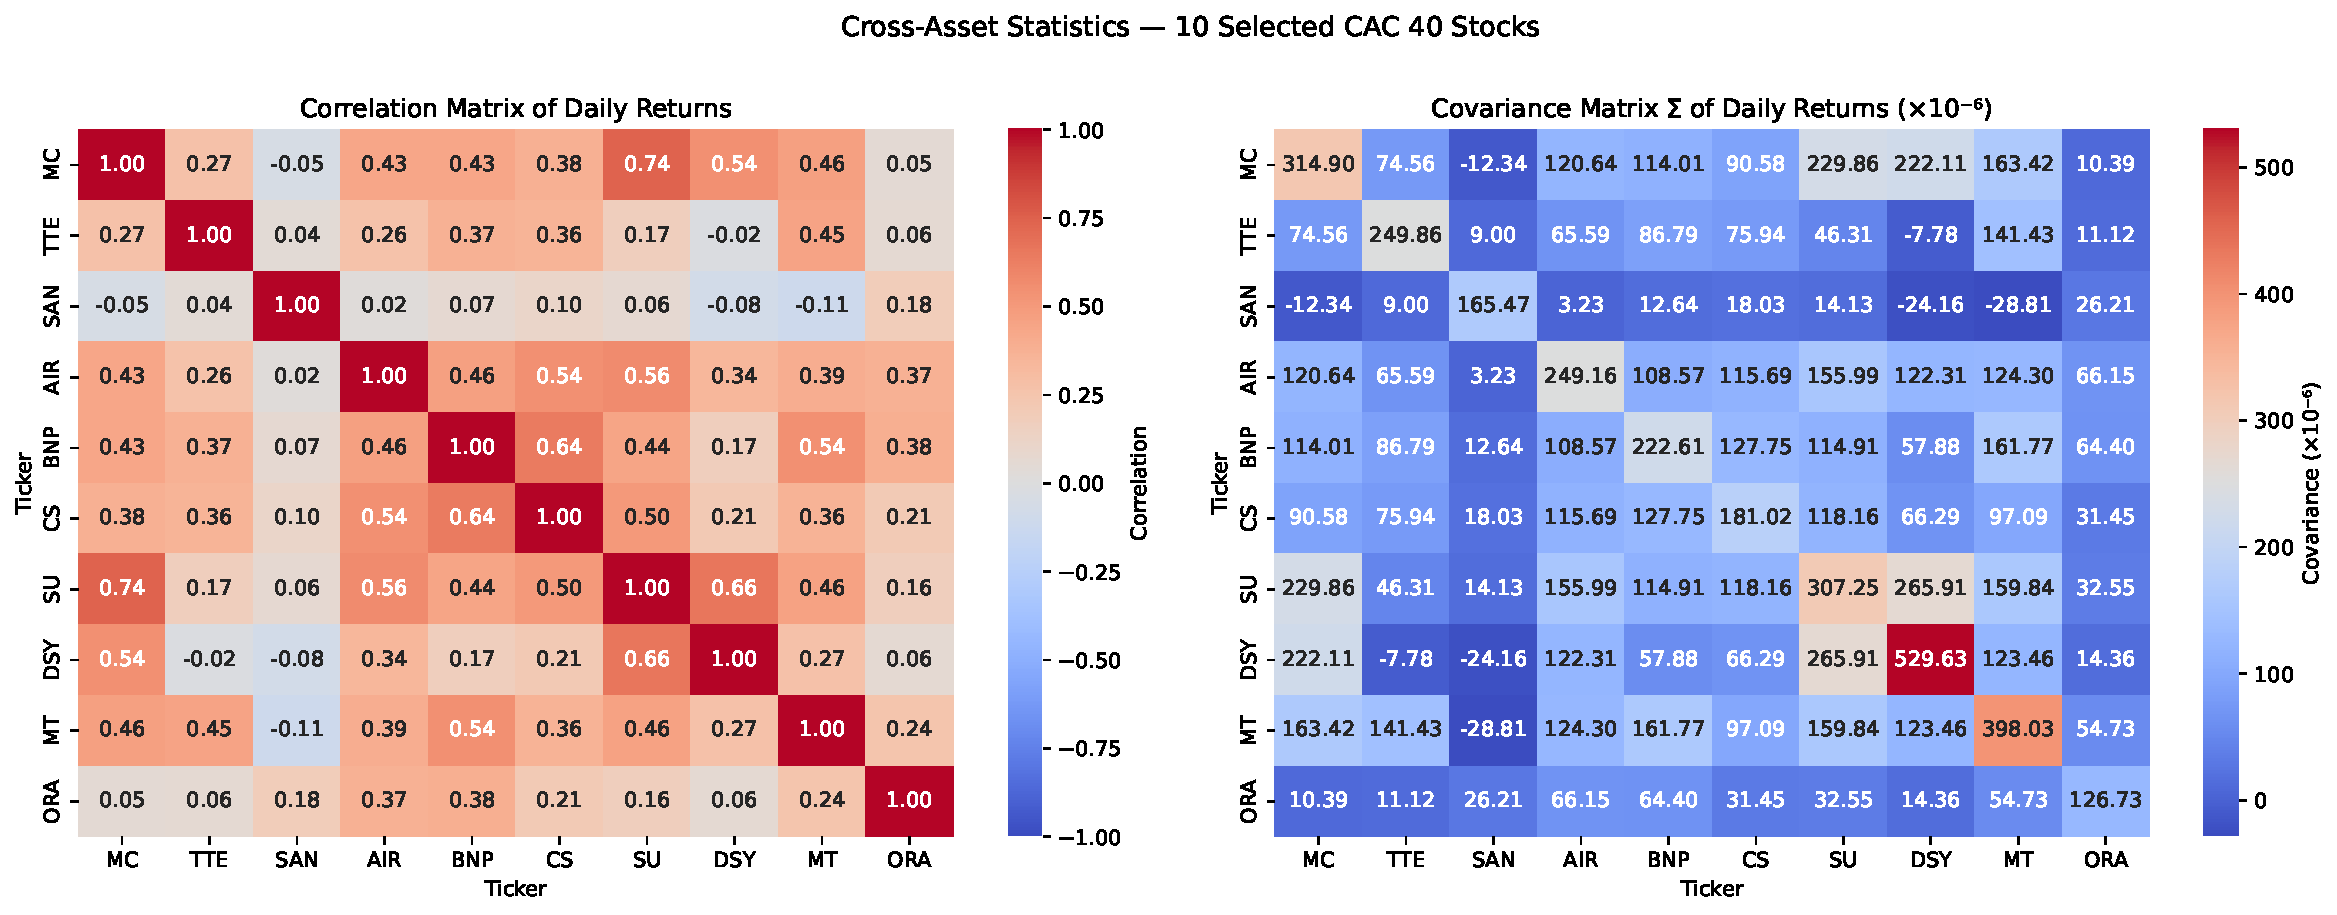
\includegraphics[width=0.96\textwidth]{fig_02_corr_cov_matrices}
  \caption{\emph{Left}: sample correlation matrix. \emph{Right}: covariance matrix
           ($\times10^{-6}$). All pairwise correlations are positive.}
  \label{fig:corr_cov}
\end{figure}

\subsection{Lag-1 Autocorrelation}

The lag-1 autocorrelation $\hat\rho_j$ is estimated for each stock (Table~\ref{tab:autocorr},
Figure~\ref{fig:autocorr}). Values lie in $[-0.168, 0.123]$: seven stocks show mean
reversion (negative, consistent with bid--ask bounce) and three show slight momentum.
Despite their small magnitude, these are the sole AR(1) predictors used for expected-return
forecasting.

\begin{figure}[H]
  \centering
  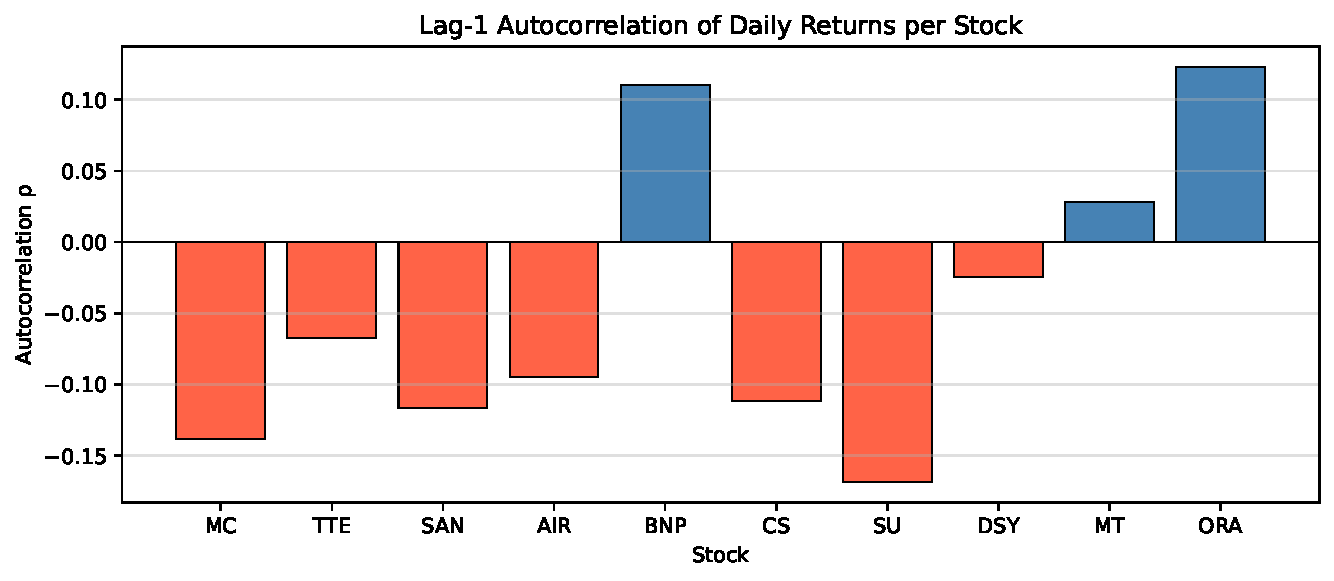
\includegraphics[width=0.65\textwidth]{fig_03_autocorrelation}
  \caption{Lag-1 autocorrelations $\hat\rho_j$. Negative: mean reversion; positive: momentum.}
  \label{fig:autocorr}
\end{figure}

\begin{table}[H]
\centering
\caption{Lag-1 autocorrelation $\hat\rho_j$ per stock.}
\label{tab:autocorr}
\small
\begin{tabular}{lrllrlr}
\toprule
Ticker & $\hat\rho_j$ & & Ticker & $\hat\rho_j$ & & \\[-2pt]
\midrule
MC  & $-0.138$ & & BNP & $+0.110$ \\
TTE & $-0.067$ & & CS  & $-0.111$ \\
SAN & $-0.116$ & & SU  & $-0.168$ \\
AIR & $-0.095$ & & DSY & $-0.024$ \\
MT  & $+0.028$ & & ORA & $+0.123$ \\
\bottomrule
\end{tabular}
\end{table}

\subsection{AR(1) Projections and Markowitz Weights}

Under a zero-mean AR(1), the expected return at day $i+1$ is
$\hat{R}_{i+1,j} = \hat\rho_j \cdot R_{i,j}$.
The Markowitz weight vector (unit-sum constraint, no leverage cap) is:
\begin{equation}
  \Omega_{i+1}
  = \frac{\Sigma^{-1}\hat{R}_{i+1}}{\mathbf{1}'\Sigma^{-1}\hat{R}_{i+1}}.
  \label{eq:markowitz}
\end{equation}
Because $|\hat\rho_j| \ll 1$ the denominator $\mathbf{1}'\Sigma^{-1}\hat{R}_{i+1}$
is near zero on most days, producing extreme leverage (Figure~\ref{fig:weights}):
time-averaged $\sum|\bar\Omega_j| \approx 22$, with individual mean weights
ranging from $-3.86$ (AXA) to $+3.54$ (LVMH).

\begin{figure}[H]
  \centering
  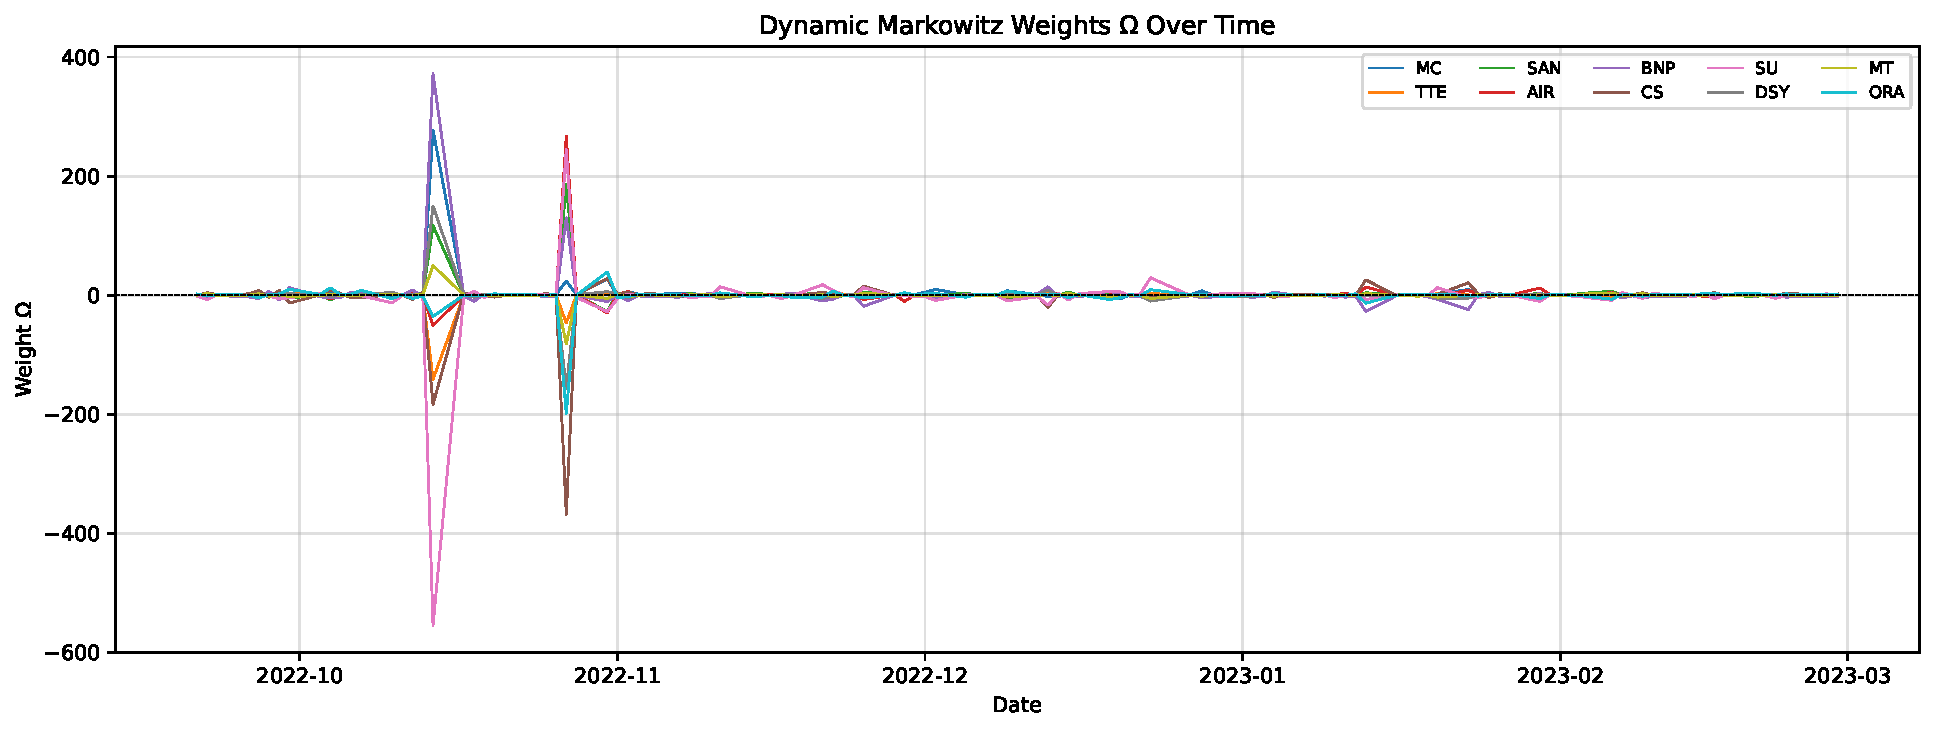
\includegraphics[width=0.92\textwidth]{fig_05_dynamic_weights}
  \caption{Daily Markowitz weights over the investment period. Extreme excursions
           arise when the AR(1) projected return is near zero.}
  \label{fig:weights}
\end{figure}

\subsection{Realised Portfolio Returns and Look-Ahead Bias}
\label{sec:bias}

The daily realised portfolio return $r_{p,i+1} = \Omega_{i+1}'R_{i+1}$ is compounded
into a cumulative value $V_{i+1} = V_i(1+r_{p,i+1})$ (Figure~\ref{fig:performance}).
The portfolio ends at $\mathbf{-1271.82}$ (base~100) versus $+122.89$ for an
equal-weight benchmark: extreme leverage turns even occasional forecast errors into
losses exceeding available capital.

\begin{figure}[H]
  \centering
  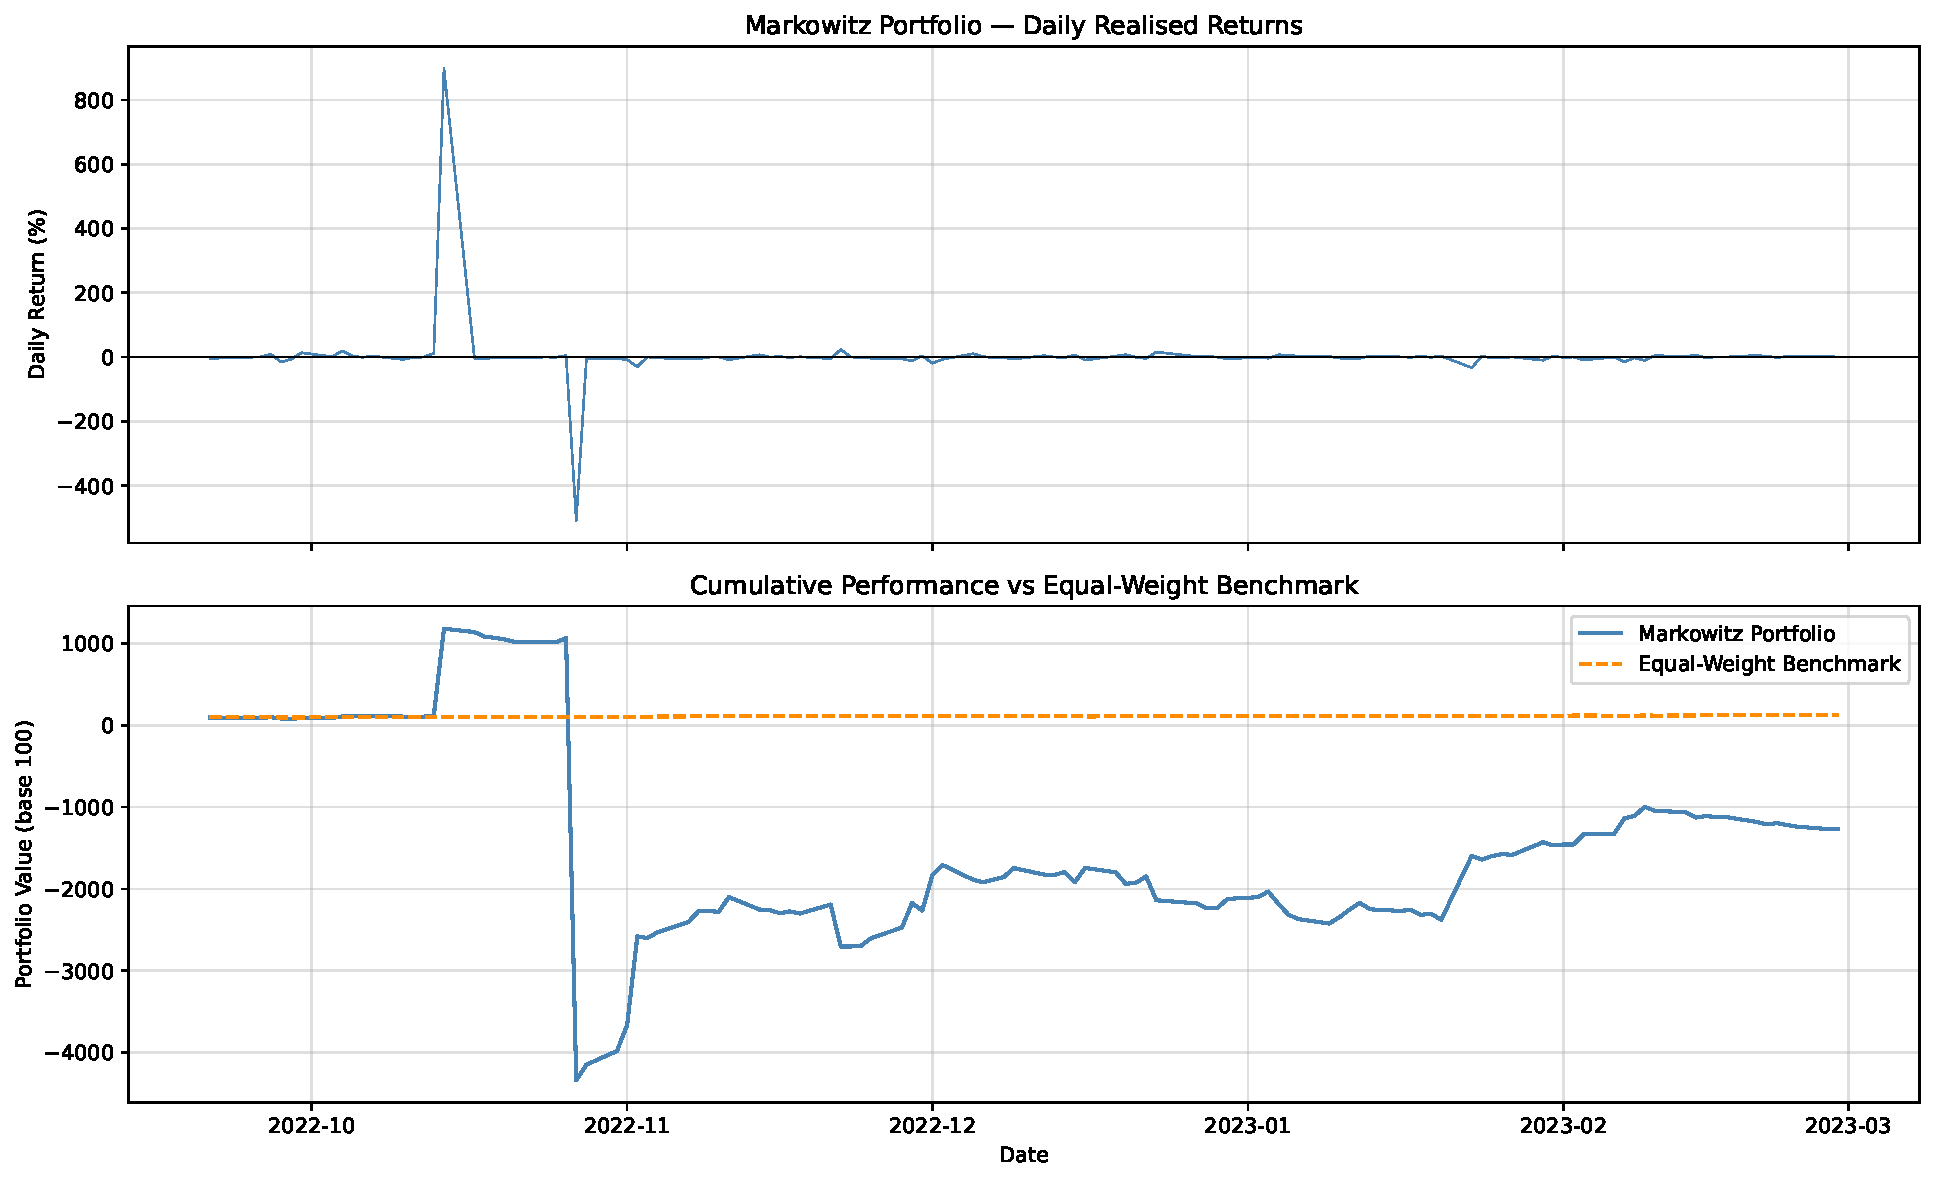
\includegraphics[width=0.92\textwidth]{fig_06_portfolio_performance}
  \caption{\emph{Top}: daily portfolio returns (range $[-507\%,\; +897\%]$).
           \emph{Bottom}: cumulative value; equal-weight benchmark shown in orange.}
  \label{fig:performance}
\end{figure}

\paragraph{Look-ahead bias.}
$\Sigma$ in \eqref{eq:markowitz} is estimated on the \emph{full} return sample,
including data future to any given trading day — a textbook look-ahead bias.
Here the bias cannot offset the absence of a real forecasting edge;
a rolling-window $\Sigma$ would reduce bias without solving the fundamental leverage problem.

% ======================== 3. RISK AND PERFORMANCE ========================
\section{Risk and Performance Evaluation}

\subsection{Sharpe Ratio}

Sharpe~$= \bar{r}_p / \sigma_p$ (risk-free rate~$= 0$). We report ex-ante (using
projected returns $\hat{r}_{p,i+1} = \Omega_{i+1}'\hat{R}_{i+1}$) and ex-post
(using realised returns).

\begin{table}[H]
\centering
\caption{Sharpe ratio of the Markowitz portfolio.}
\label{tab:sharpe}
\small
\begin{tabular}{lcc}
\toprule
Variant & Daily SR & Annualised ($\times\!\sqrt{252}$) \\
\midrule
Ex-ante  & $0.0604$ & $0.9595$ \\
Ex-post  & $0.0277$ & $0.4394$ \\
\bottomrule
\end{tabular}
\end{table}

The ex-ante SR of $0.96$ is by construction the maximum achievable from the AR(1)
signal. The realised SR drops to $0.44$: only $\approx 46\%$ of the constructed
signal survives in actual returns, a direct consequence of the low autocorrelation
magnitudes. Both figures correspond to a daily standard deviation $\approx 97\%$
(extreme leverage), making conventional Sharpe interpretation problematic.

\subsection{Upside Potential Ratio}

\[
  \mathrm{UPR}
  = \frac{\mathbb{E}[\max(r_p,0)]}{\sqrt{\mathbb{E}[\min(r_p,0)^2]}}
  = \frac{0.212}{0.655} = 0.323.
\]
The UPR well below~1 confirms heavily left-skewed returns: average losses ($0.655$
per losing day) outweigh average gains ($0.212$) by a factor of~3. Leverage amplifies
forecast errors disproportionately — when the AR(1) signal is wrong on a large
market move the loss is multiplied by the full $22\times$ leverage.

\subsection{Maximum Drawdown}

\[
  \mathrm{MDD} = -467.4\%, \quad
  \text{Peak: 14~Oct~2022}, \quad
  \text{Trough: 27~Oct~2022.}
\]

\begin{figure}[H]
  \centering
  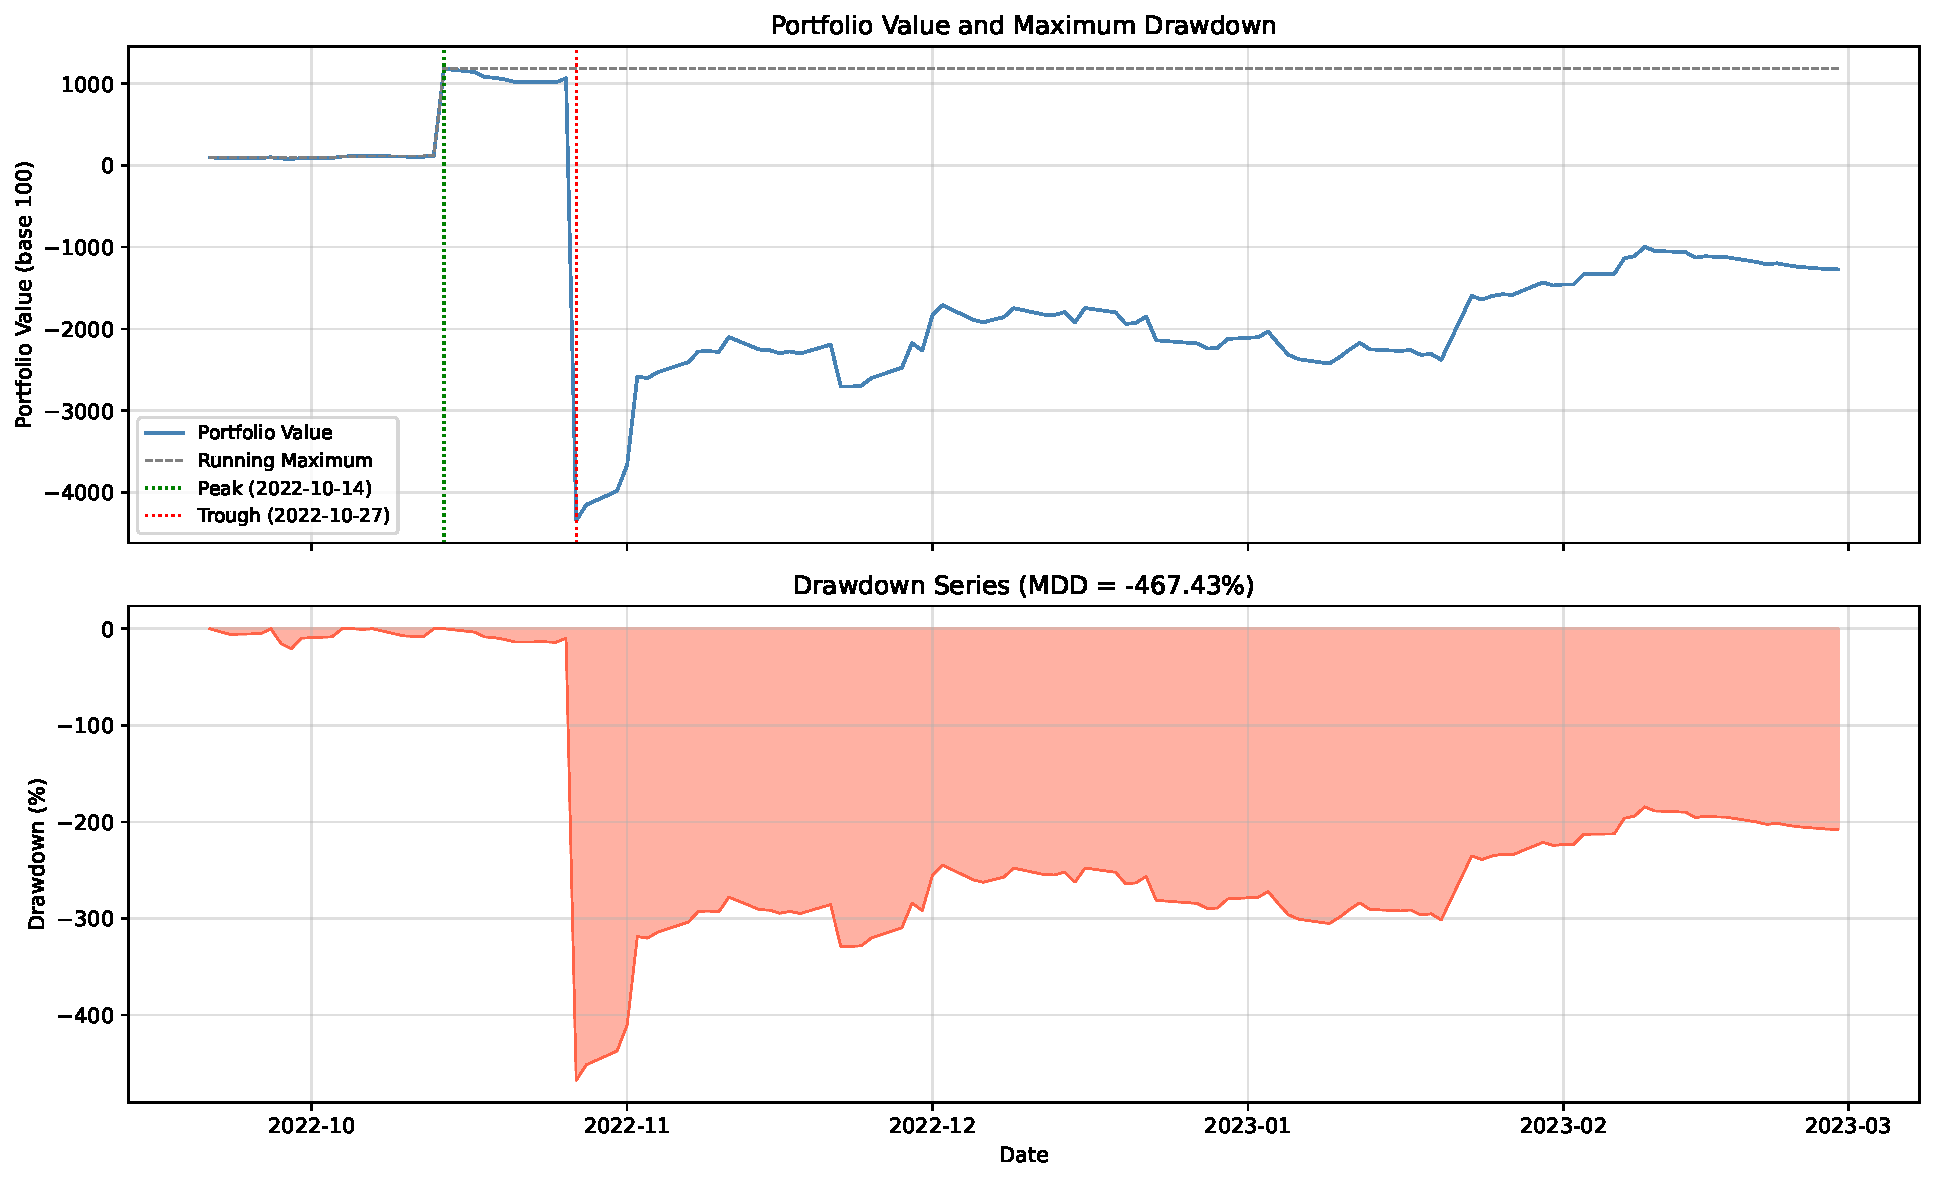
\includegraphics[width=0.92\textwidth]{fig_07_drawdown}
  \caption{Cumulative value (top) and drawdown series (bottom).
           Peak ($+1181$, green) and trough ($-4340$, red) are marked.}
  \label{fig:drawdown}
\end{figure}

The MDD exceeds $-100\%$ because the portfolio value becomes deeply negative.
The critical two-week window (14--27~Oct~2022) coincided with peak Q4~2022
European market stress (BoE emergency gilt intervention, ECB tightening climax,
energy-price spike). Large intraday reversals during this period caused the AR(1)
projections to be systematically wrong, and extreme leverage converted these
errors into catastrophic losses.

\subsection{Additive Volatility Contributions}

\begin{equation}
  \sigma_p = \sum_{j=1}^{10} C_j, \qquad
  C_j = \frac{\bar\Omega_j \cdot (\Sigma\bar\Omega)_j}{\sigma_p},
\end{equation}
evaluated at the time-averaged weight vector $\bar\Omega$ (Table~\ref{tab:vol},
Figure~\ref{fig:vol_contrib}).

\begin{figure}[H]
  \centering
  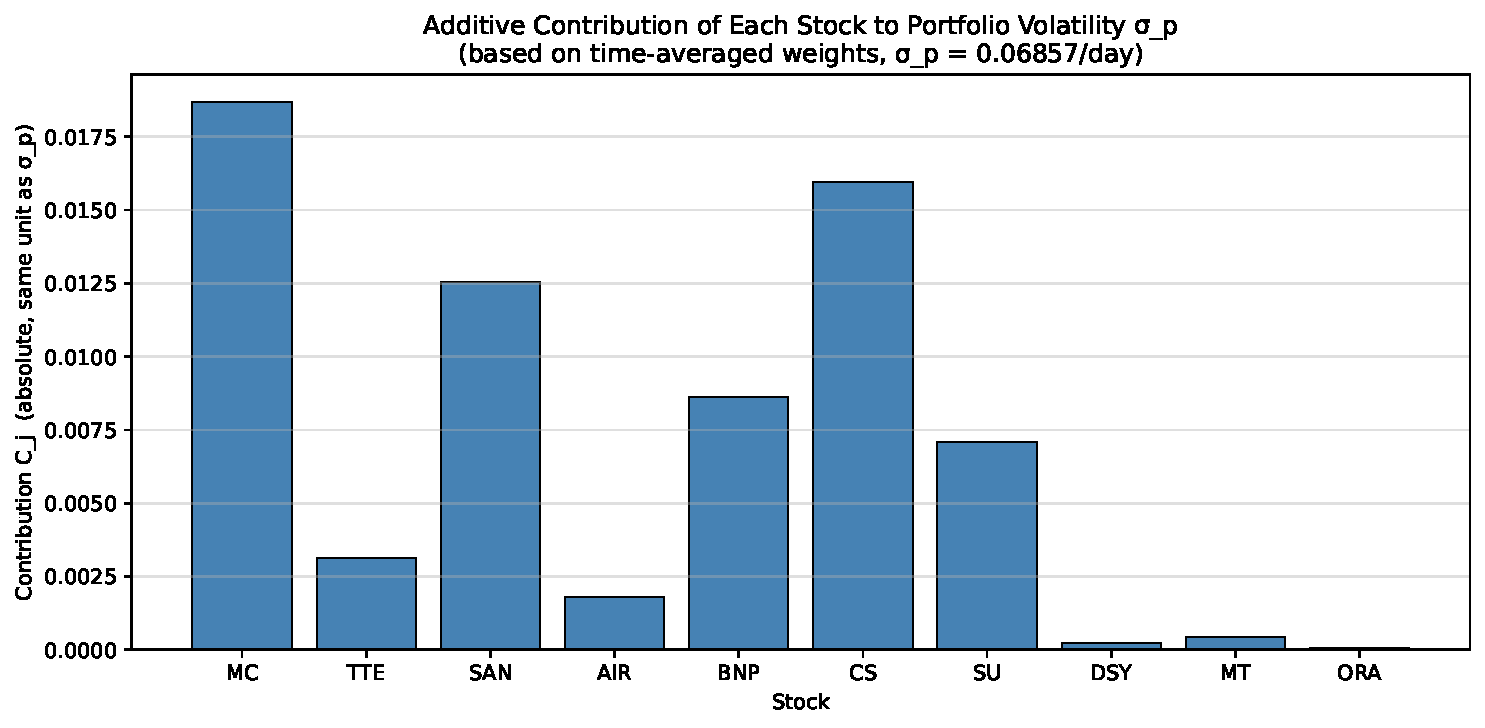
\includegraphics[width=0.72\textwidth]{fig_08_vol_contributions}
  \caption{Additive contribution $C_j$ per stock to portfolio daily volatility
           $\sigma_p = 0.0686$ (all positive, even short positions).}
  \label{fig:vol_contrib}
\end{figure}

\begin{table}[H]
\centering
\caption{Volatility decomposition at time-averaged weights
         ($\sigma_p = 0.0686$/day, annualised $1.089 = 108.9\%$/year).}
\label{tab:vol}
\small
\begin{tabular}{llrrr}
\toprule
Ticker & & $\bar\Omega_j$ & $C_j$ & Share \\
\midrule
MC  & LVMH               & $+3.538$ & $0.01868$ & $27.24\%$ \\
CS  & AXA                & $-3.855$ & $0.01596$ & $23.27\%$ \\
SAN & Sanofi             & $+2.773$ & $0.01255$ & $18.30\%$ \\
BNP & BNP Paribas        & $+3.055$ & $0.00862$ & $12.57\%$ \\
SU  & Schneider Elec.\   & $-3.261$ & $0.00709$ & $10.35\%$ \\
TTE & TotalEnergies      & $-1.338$ & $0.00313$ & $ 4.57\%$ \\
AIR & Airbus             & $+1.973$ & $0.00181$ & $ 2.63\%$ \\
MT  & ArcelorMittal      & $-0.362$ & $0.00045$ & $ 0.65\%$ \\
DSY & Dassault Syst.      & $-0.143$ & $0.00024$ & $ 0.35\%$ \\
ORA & Orange             & $-1.378$ & $0.00004$ & $ 0.06\%$ \\
\midrule
    & \textbf{Total}     &          & $0.06857$ & $100.0\%$ \\
\bottomrule
\end{tabular}
\end{table}

Annualised portfolio volatility is $108.9\%$ vs.\ $\approx 12$--$16\%$ for individual
stocks. Risk is concentrated in three names (MC + CS + SAN~$= 68.8\%$) and,
crucially, \textbf{all $C_j > 0$} including short positions. Because all pairwise
correlations are positive, short positions still move together with the portfolio in
the direction of their own weight --- there is no true hedging effect.

% ======================== 4. CONCLUSION ========================
\section{Conclusion}

Seven key findings:

\begin{enumerate}[leftmargin=2em,label=(\roman*),itemsep=1pt,topsep=2pt]
  \item All pairwise correlations positive (avg~$0.29$); Sanofi and Orange are the
        weakest-linked, most defensive names.
  \item AR(1) autocorrelations in $[-0.168, 0.123]$: seven mean-reverting, three momentum.
        Signals are near-zero and noise-dominated.
  \item Unconstrained Markowitz amplifies near-zero forecasts into $22\times$ leverage,
        the root cause of all subsequent failures.
  \item Ex-ante SR~$0.96$ vs.\ ex-post SR~$0.44$ (annualised): only 46\% of the
        optimised signal materialises in realised returns.
  \item UPR~$= 0.32$: losses outweigh gains 3-to-1 in a left-skewed, leveraged distribution.
  \item MDD~$= -467\%$, portfolio ends at $-1272$ (base~100); worst episode triggered
        by Q4~2022 European market stress.
  \item All ten volatility contributions are positive: no genuine diversification in an
        all-positive-correlation universe under unconstrained weights.
\end{enumerate}

\paragraph{Remedies.}
Two straightforward improvements would transform this from a mathematical exercise into
a deployable strategy: (i)~\textbf{leverage/position constraints} ($|\Omega_j|\le 0.2$)
to prevent weak signals from generating extreme bets; and (ii)~\textbf{Ledoit--Wolf
covariance shrinkage} to dampen $\|\Sigma^{-1}\hat{R}\|$ when $\hat{R}$ is small.

\smallskip\noindent
\textit{Code: all computations are in the accompanying notebook \texttt{main.ipynb}.}

\end{document}
